
\documentclass{article}% use option titlepage to get the title on a page of its own.

\linespread{1.4}

\usepackage{lmodern}
\usepackage{listings}
\usepackage{color}

\definecolor{dkgreen}{rgb}{0,0.6,0}
\definecolor{gray}{rgb}{0.5,0.5,0.5}
\definecolor{mauve}{rgb}{0.58,0,0.82}

\usepackage{graphicx}
\graphicspath{ {./images/} }



\title{%
  Non-negative LASSO \\
  \large A Portfolio replication application}

\date{2019, February}
\author{Giovanni Misseri, Andrea Della Vecchia \\ \\ 
Business Economics and Financial Data}
\begin{document}
\maketitle
\tableofcontents
\newpage
\section{Introduction}

Portfolio management has always been one of the most used way investors start approaching to financial investments. An important task in finance is indeed optimizing the revenue with respect to the risk of investing in a portfolio.

Markowitz in the '50, stated that single minded pursuit of high returns results in a poor strategy and rational investors need to balance their desire for high returns with low risk. So investing in a portfolio seems reasonable, indeed it diversify our investment and if we are able to spot profitable companies on which invest, we are guaranteed good revenue taking relatively low risk.
\\

There are mainly two strategies in portfolio management, active and passive managements. Active management tries to exploit the fluctuations of the market to gain as much as possible. On the other hand, passive management, tries to mimic the performance of an index. As one can easily notice, with active approach it's possible to loose great amount of money even investing on, on average, growing companies. On the other hand if we are able to well mimic a, on average, growing index, with passive approach we are guaranteed positive revenue.

Empirically is often the case that passive approach outperforms active approach, also due to the transaction costs. In this work we will propose two different solutions to pursue respectively the passive and the active approach.

\newpage
\section{Shrinkage Methods}

If we have a feature or some measurements of an interesting phenomenon, is often the case that, given some related variables, we try to explain the phenomenon as a function of the related variables. The use of linear model, in case of linear relation between phenomenon and variables, is a good choice for two reasons: it gives good prediction and on the other hand it's highly interpretable. 

In general the more correlated variables we have, the "better" the model will be; but sometimes the presence of too much independent variables conditions the prediction error, and also the presence of an high number of predictors limits the interpretability of the model. For these reasons one could decide to add a regularization term to its minimum least square problem.

\[
\min_{\beta_0 , \beta} \frac{1}{N} \sum_{i=1}^N (y_i-\beta_0 - \sum_{j=1}^p x_{ij}\beta_j)^2 + \lambda\sum_{j=1}^p |\beta_j |^q 
\]

Where $|\beta|^p$ is the $p$-norm of $\beta$.
\\

If in the regularized minimization problem we choose norm-two we obtain the ridge regression, if we choose the norm-one we obtain LASSO regression. 


It's easy to prove that shrinkage methods also solve an other type of problem related to ordinary least square. With OLS indeed the solution of the minimization problem is $ \beta_{ols}=(X^TX)^{-1}X^Ty$, decomposing $X$ through SVD, $X=V\Sigma U^T$, we get $\beta_{ols}=U\Sigma^{-1}V^Ty$. From this we can easily see that if $\Sigma$ is not invertible $\beta_{ols}$ could not be found.
\\

Shrinkage methods deal with this problem. Ridge regression ends up giving $\beta_{ridge}=U(\Sigma^2+\lambda I)^{-1} \Sigma V^T y$. Lasso regression's beta cannot be written in an explicit form, but the non-invertibility problem is solved due to the fact that, fixed $\lambda$, at the optimum, some beta will be equal to zero. Intuitively this is due to the feasible solutions space shape; indeed LASSO regression can be written as the following minimization problem.
\begin{equation}
 \min_{\beta} \sum_{i=1}^N ( y_i -\beta_0 -\sum_{j=1}^p x_{ij} \beta_j)^2 ~~subject~to~\sum_{j=1}^p |\beta_j| \leq t
\end{equation}

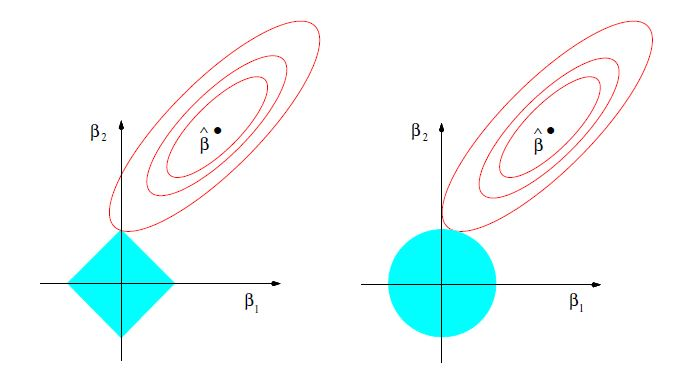
\includegraphics[scale=0.75]{lasso}

\subsection{LASSO and Portfolio Replication}

A replicating portfolio for a given asset or series of cash flows is a portfolio of assets with the same properties. So the principal problem of building a good replicating portfolio for a certain financial aggregate index is finding the right components of the index, the one able to represent the index itself. 

With the problem posed like that, the link between lasso regression and portfolio replication it's evident. Indeed one interesting properties of lasso regression is the variable selection consistency, so using lasso regression we are guaranteed, under certain condition, that it will select an optimal subset of variables in order to explain our dependent variable. It's clear now that lasso could help on the selection of the subset of time series that will be part of the portfolio; so we will select a subset of an index' components  able to explain the index itself.
\\

Here comes one problem, how to use lasso, a cross-sectional regression method, on a dynamic dataset? We will use a moving window approach, so we will assume that the data inside a window of fixed length are time invariant, and we compute lasso on that.

Another problem is the interpretation of the resulting model. Ones we find the solution to the lasso minimization problem, we have the beta related to all the variables, in our case the components of the index. Some beta will be equal to zero, so they will be excluded by our portfolio, for all the other beta a nice interpretation is available. 

If we carefully think to lasso as it has been defined in $(1)$, we approximate an index, the used one will be $Sp500$, as a function of some of it's components, conditioning to the fact that the sum of the associated beta is less than a given $t$. Practically we will work on the daily log-returns, and so our response and regressors will be all daily log-return; said that it's easy to see that $t$ can be seen as the initial budget and each beta is the volume of the "suggested" investment in a certain asset to do in order to replicate the index performances. Later on we will exploit this fact to run simulations using the different proposed methods.

For an active approach everything works fine, a positive beta will be an investment and a negative beta will be a short sell. On the other hand, for passive approach, it could be forbidden or in general doesn't make much sense to use short sell. For this reason to our estimates we need to add the constrain of non-negativity.

Considering that also elastic net regression has the consistency variable selection, we will try to select the assets both with lasso and elastic net regression. Some comparison will be done on that.

\subsection{Dataset Analysis}
\begin{figure}[h!!!]
  \centering
  \includegraphics[scale=0.6]{daily_var.png}
  \caption{Daily values of $Sp500$ index}
  \label{daily_var}
\end{figure}

The major problem dealing with this kind of financial data is the high variability of the index from one day to another. In our case, this means that the behaviour of  $Sp500$ at time $t+1$ is very difficult to predict at time $t$.
We start our analysis with the simpler case in which we want to replicate $Sp500$ at time $t$ knowing the values of the $500$ assets (our $x$ variables) composing the index. Since there will be some correlation between the assets we can ask ourselves how many of them are really needed. Keeping the number of variables low is not only useful for having a less complex model but also, if we want really to invest in the assets and reproduce the index, to avoid the payment of a large number of fees (one for each purchase). On the other hand, the more we simplify the model ignoring some variables, the more our replication of the index will result to be inaccurate. With Lasso we can control the number of variables different from $0$ adjusting the value of the regularization parameter $\lambda$, we show the results below: 

\begin{figure}[h!]
  \centering
  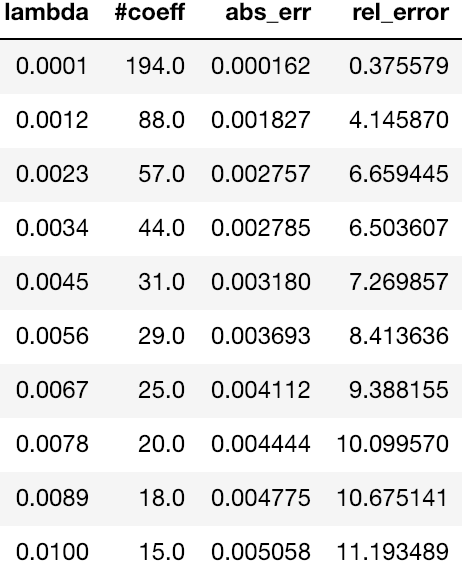
\includegraphics[scale=0.6]{err_lambda.png}
  \caption{$Sp500$ replication varying $\lambda$}
  \label{err_alpha}
\end{figure}

Unfortunately, this is not very useful. At time $t$ we are interested in predicting $Sp500$ at time $t+1$ and according to that planning our financial strategy. The simplest way to do it is by using our linear model shifting $y_t$ by a step $h$ with respect to $x_t$:
\begin{equation}
 \min_{\beta} \sum_{t=1}^T ( y_{t+h} -\beta_0 -\sum_{j=1}^p x_{tj} \beta_j)^2 ~~subject~to~\sum_{j=1}^p |\beta_j| \leq C.
\end{equation}

As mentioned before, due to the high variance of the process this naive approach is quite inefficient and this will be a problem in the following sections where we will try to build up a financial strategy based on these predictions.

\iffalse
\begin{figure}
  \begin{subfigure}[b]{0.35\textwidth}
    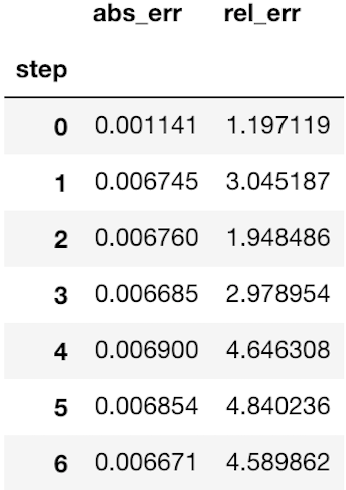
\includegraphics[width=\textwidth]{err_step.png}
    \caption{Picture 1}
    \label{fig:1}
  \end{subfigure}
  %
  \begin{subfigure}[b]{0.6\textwidth}
    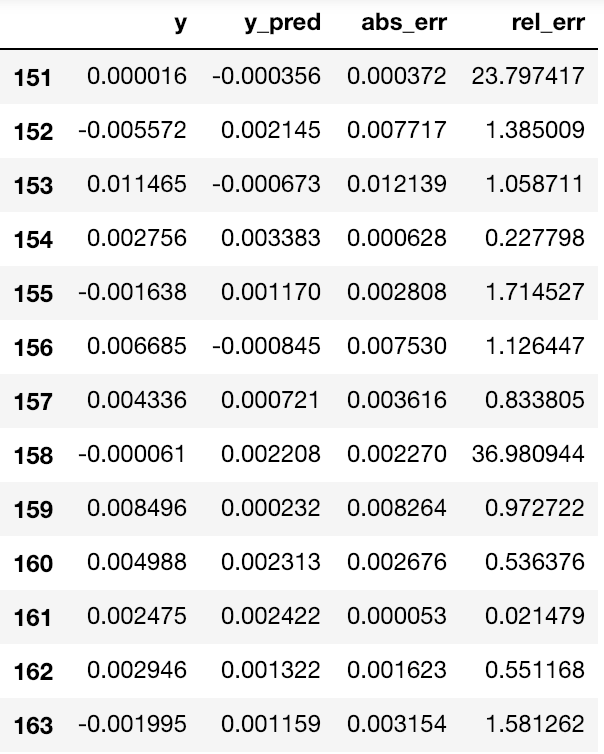
\includegraphics[width=\textwidth]{pred_step1.png}
    \caption{Picture 2}
    \label{fig:2}
  \end{subfigure}
\end{figure}
\fi

\begin{figure}[h!]
  \centering
  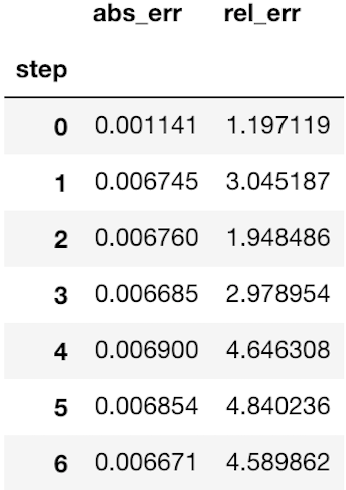
\includegraphics[scale=0.55]{err_step.png}
  \caption{Accuracy in predicting $y_{t+h}$ given $x_t$ }
  \label{err_step}
\end{figure}

\begin{figure}[h!!!]
  \centering
  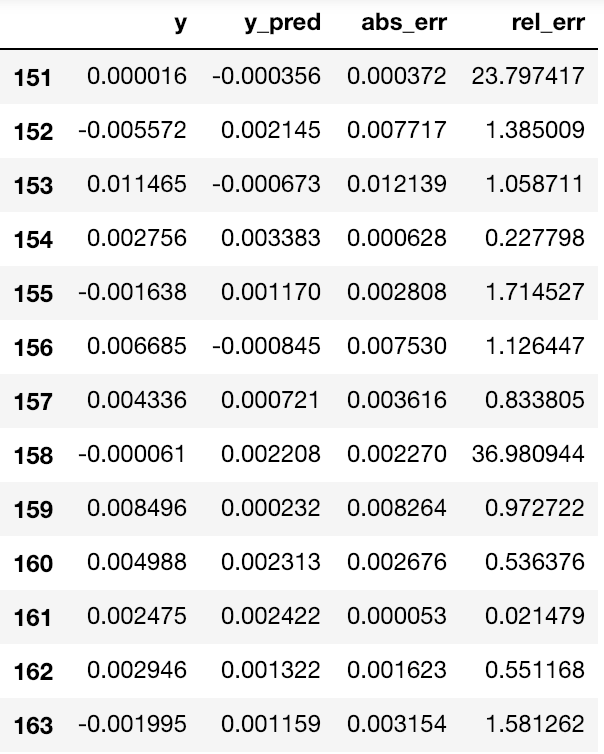
\includegraphics[scale=0.55]{pred_step1.png}
  \caption{One-step ahead prediction}
  \label{err_step}
\end{figure}




\subsection{Parameter estimation}
As we said our principal aim is to replicate the $Sp500$ with a relatively low number of assets. To select the right one we could use, as explained in previous paragraphs, lasso or elastic net regression; now we have to deal with the parameter estimation.

As we said before, since  $Sp500$ is just a combination of 500 assets, we suppose that it has a linear relation with the selected assets. A first and natural choice for the $\beta$ of the model are the one obtained by the non-negative lasso regression or non-negative elastic net regression on the whole set of $Sp500$ constituents. Actually this gives nice results, but we will see in experimental phase that selecting the assets and than estimate the model using non negative OLS works even better. 
\\

We will use a moving window approach to build the models for both passive and active portfolio management. It's clear in fact that the size of the used window will affect all the further analysis. After different tests, presented before, we decided to use a window 250 observation long. In this way we end up having enough data to build meaningful models, but not too much, because we want to preserve the time invariance of the data inside the window.





\newpage
\section{Portfolio replication}
In this section we will present the two developed strategies to manage the portfolio. 
One of  the principal aim of portfolio management is the replication of a certain index performance, using only a relatively small number of assets. This is justified by the fact that a portfolio with 50 assets is much more flexible and easy to manage with respect to the one with 500 assets. Also an other good reason is that, depending of the type of taxation, could be necessary to pay a fixed amount of fee for each asset we decide to invest on. So if we are able to find a small subset of the 500 assets able to guarantee similar performances, we will gain in terms of management simplicity and lower taxation.

\subsection{Beta}
Using a moving window of length $250$ and using an appropriate regularization parameter $\lambda$ in order to have a number of variables (i.e number of $\beta$-parameters to estimate), we obtain the following result:
\begin{figure}[h!]
  \centering
  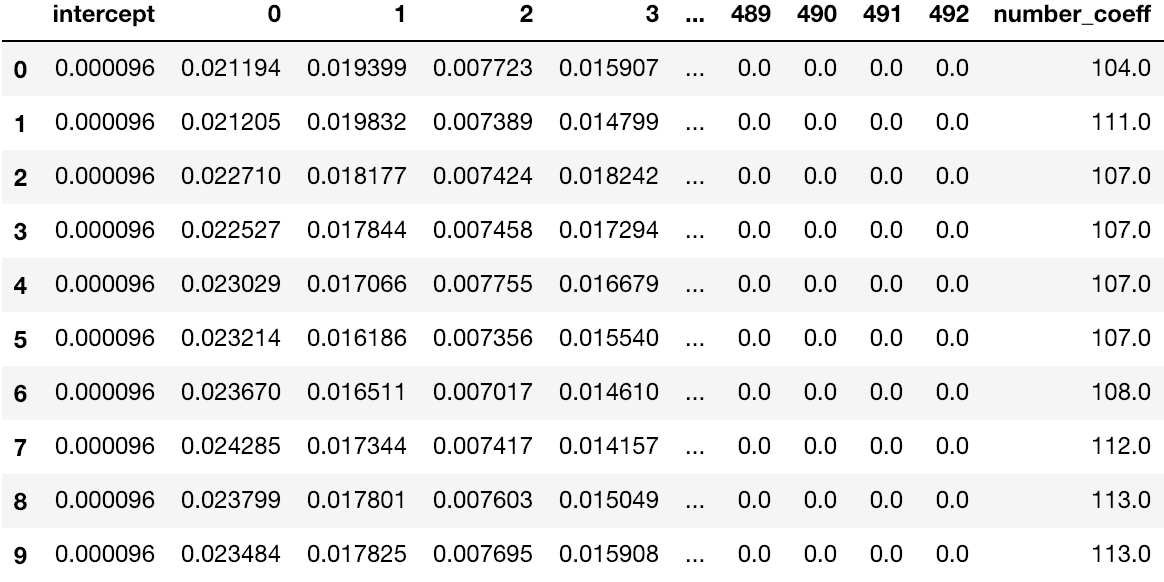
\includegraphics[scale=0.6]{beta_dataset.png}
  \caption{Intercept and $\beta$-coefficients predicted by our model}
  \label{beta_dataset}
\end{figure}
We want to understand how rapidly these $\beta$-parameters change, in particular the turnover among the variables and, in case the model trained in the window$[t+1:t+251]$  introduce a new variable with respect to the model trained in the window$[t:t+250]$, which is the weight of this new variable inside the model (and vice versa for a variable leaving the model). What we get is that on average only $5.49$ new variables are added to the new model (circa $4\%$) and $5.47$ are removed (circa $4\%$). Moreover, new assets enter the model with really low weight (so they still are almost irrelevant) and on the other hand leaving variables are unsurprisingly among the least important in the previous model. In fact, the mean value of the $\beta$-coefficients of the new variables is $0.000858$ (compared with a $0.006668$ mean value of all the $\beta$-coefficients of the chosen variables, only the $0.12\%$ of the chosen variables has a lower weight). We have a similar result also for the variables leaving the model.
\begin{figure}[h!]
  \centering
  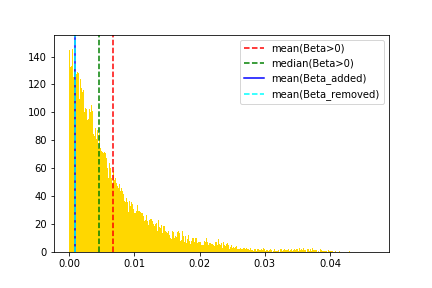
\includegraphics[scale=0.6]{turnover.png}
  \caption{Relevance of the added/removed variables inside the model}
  \label{turnover}
\end{figure}
These results show that we can assume that our "relevant" variables, the ones chosen by our Lasso model at time $t$, will probably still be the important ones at time $t+1$ due to the fact that the only few turnovers we have are among the least important assets.


\subsection{Passive approach}

With passive approach, given that one tries to choose a growing index, we want to mimic as much as possible the index itself, in order to have its same performances.
We will work with $Sp500$, below we report the $Sp500$ time series.
\\


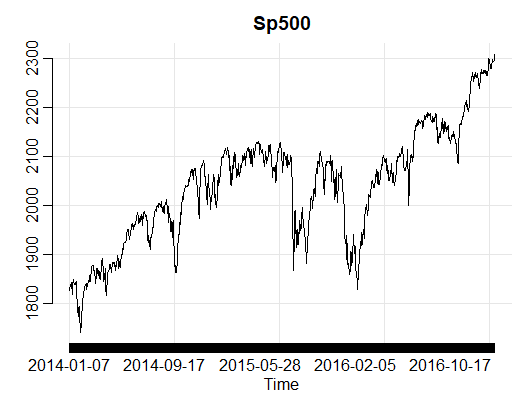
\includegraphics[scale=0.75]{sp500}
\\
		
As it's clear by the plot, the considered index, on average, grows with time, so we would have been able to perform just like the index also our portfolio would have increased its value.
\\

In previous paragraphs we already underlined how we could use Lasso in order to select the right subset of asset. So our passive approach to portfolio replication problem will be handled using lasso or elastic net.

A first way to build the portfolio is to use non negative lasso regression on the starting window, representing the time at which one decides to starts to invest, and distribute the budget proportionally to the $\beta_{lasso}$.. Given that we will work on daily log-returns, $\log(x_t)-\log(x_{t-1})$, both on dependent and independent variable. It's easy to see that $\exp(y_t)$, where $y_t$ is the response variable ($Sp500$), it's equal to the proportional value of $Sp500$ with respect to the value it take one lag before. For this reason, estimated the model on the first 250 observations, we can get the value of our portfolio after $t$ day from our investment as $\exp(\sum_{i=1}^t \hat{y_i})$, where $\hat{y}$ is the model's predicted value of the observation at time $250+i$.

For this reason becomes computationally easy to calculate the gain of a passive approach to portfolio management. 
\\

Said that we can actually report the result of the passive approach to the studied problem.

For all the further presented simulations we will use for our analysis the daily log-return of the $Sp500$ and its components form $07-01-2014$ until $09-02-2017$ (notice that some entries are missing, this is due to not collected data). So we will start using the window made by the first 250 observations of our series and building a model using non negative lasso. As we said our aim here is to reduce the number of explanatory variable of the model; due to construction reason the best choice for $\lambda$ would be 0, in fact with all the 500 components we can perfectly explain $Sp500$. So we will choose our lambda in order to have a good trade-off between number of variables kept and prediction error. 
\\


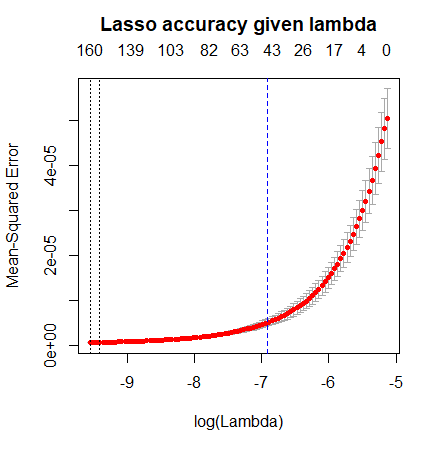
\includegraphics[scale=0.75]{lassoplot}
\\

The one reported above is the plot of the mean squared error value given a range of lambda going from $4.5$x$10^-5$ to $0.007$\footnote{The inconsistency between the lambda chosen here and in the previous sections is caused by the slightly different objective functions implemented in packets \textit{sklearn.Lasso} (Python) and  \textit{glmnet} (R) (the first one is normalized by the window length). This is not a problem since we are not interested in the value of lambda but in the number of variables chosen by the model.}. The blue line shows the selected value for $\lambda$, $0.001$. This choice seems to be a good compromise between mean squared error and number of selected variables. Indeed the chosen $\lambda$	guarantees small error being just before its explosion, and on the other hand empirical test on the moving window says that, with that lambda, we select on average 51 assets. So seems reasonable to use it. 
\subsubsection{Simulations}

\subparagraph{Non negative Lasso}
For the first simulation we will obtain our portfolio using non negative lasso. At this point we will invest in each asset proportionally its $\beta$. 

Doing like that and calculating the relative value of the portfolio after 558 days, so keeping the same portfolio for the whole time period considered, we obtain that our portfolio now worth  1.191 times or initial portfolio, so we would have gained the $19,1\%$ percent of our initial investment. Below we report the result of the simulation.
\\
\begin{center}
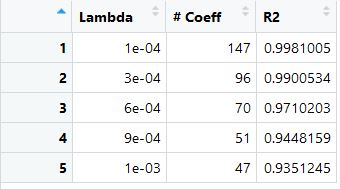
\includegraphics[scale=0.75]{tablasso}
\\

\end{center}


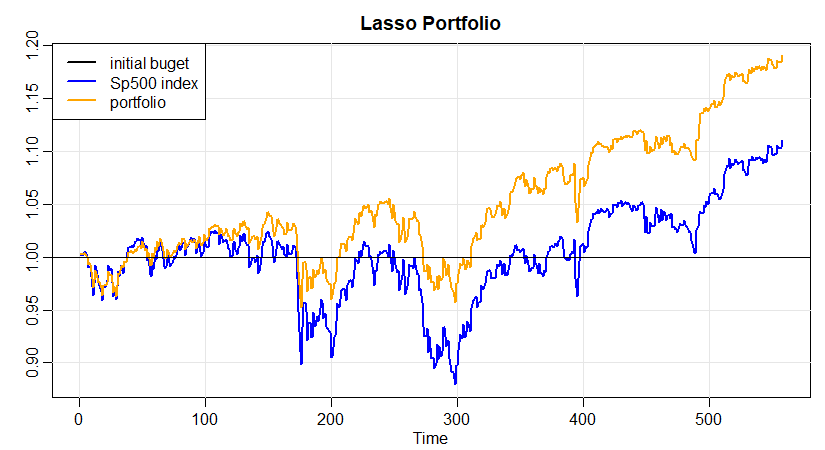
\includegraphics[scale=0.60]{lassoportfolio}
\\


%\begin{figure}[h!]
%  \centering
%  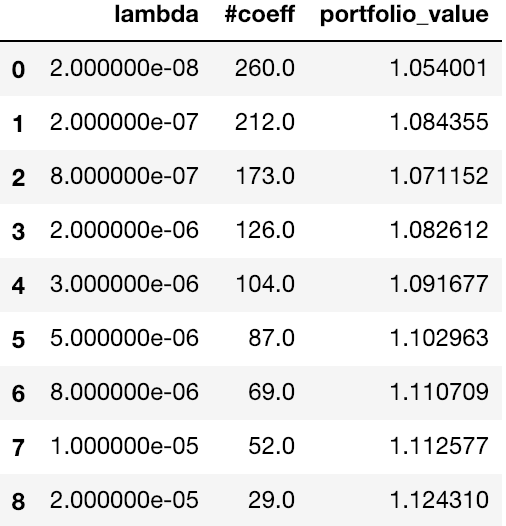
\includegraphics[scale=0.6]{portfolio_alpha.png}
%  \caption{Portfolio's revenues varying $\lambda$}
%  \label{portfolio_alpha}
%  \end{figure}
  
%\begin{figure}[h!]
%  \centering
%  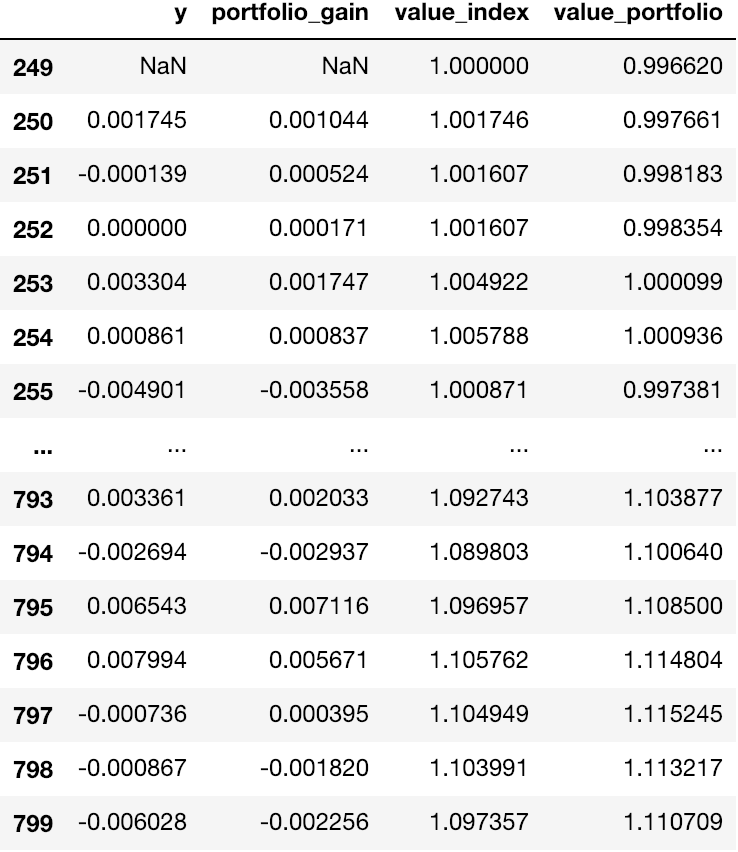
\includegraphics[scale=0.6]{portfolio_pass_es.png}
%  \caption{Portfolio's evolution with 69 variables}
%  \label{portfolio_alpha}
%   \end{figure}
   
%  \begin{figure}[h!]
%  \centering
%  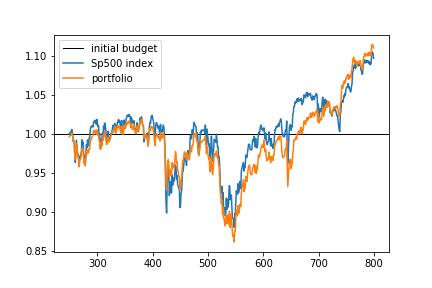
\includegraphics[scale=0.6]{pass_portfolio.png}
%  \caption{Portfolio's evolution compared with $Sp500$}
%  \label{portfolio_alpha}
%  \end{figure}

So from the figure above we can see that our portfolio follows the $Sp500$ index really well initially and then, as the time passes, it differentiates from it. This is due to the fact that the model coefficient are not static in time and so even if we estimated a good model it is valid only for a fixed period. This fact underlines the need of update the beta coefficients after a while. At the end of this simulation we gain $8.1\%$ more than the real index, so not a good approximation of the index but we selected the assets that on average grew more than the market.

\subparagraph{Non negative Elastic Net}
Non negative lasso seems to work pretty well, but as we can see from the picture above happen that our portfolio value is quite different from the $Sp500$ index, surely this can bring advantages if one decides to exit from the market in a moment in which he is earning more than the general index, but also the opposite situation is equally likely. So we would like to stick as much as possible to the index.

If one thinks to the data we are working on, actually can happen to have an asset that is not really growing with time nor decreasing. This situation creates assets with very low variance and it brings to distorted model's coefficient for that specific asset. For this reason, also due to what we said in chapter (2), adding a ridge constrain to our minimization problem can help finding better beta.

Adding a ridge constrain ends up being elastic net regression. As for lasso, also here we will work only on non negative coefficient.
\\

The general behaviour when varying the $\lambda$ value is the same as before;the behaviour of the portfolio time series varying the $\alpha$ parameter is interesting. $\alpha$ represents on which percentage the $l$-1 regularization enters in the minimization problem, $1-\alpha$ will be the percentage the ridge regularization enters. In fact keeping almost constant the number of coefficients, adjusting properly $\alpha$ and $\beta$, the result is almost the same. So seems much more important the number of assets one uses with respect the $\alpha$ and $\beta$ parameter.
\\

Below the plot containing the simulation results using non negative elastic net.
\\

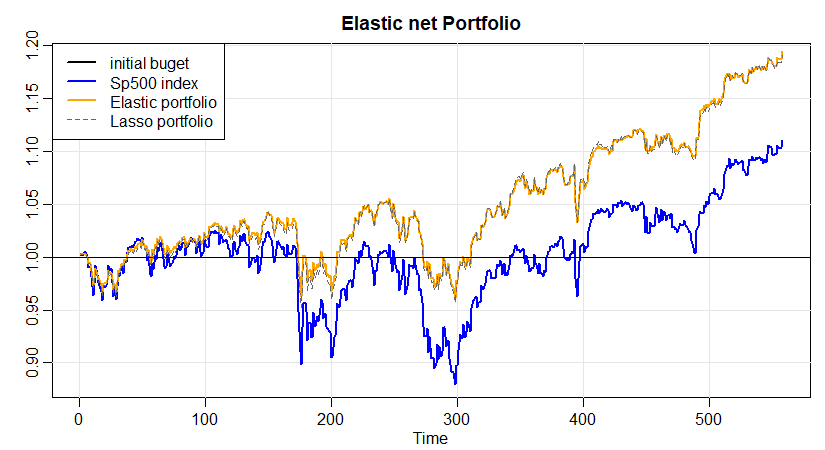
\includegraphics[scale=0.60]{elasticportfolio}
\\

So it's clear that the two results are absolutely comparable. In the case reported above we used for elastic net $\lambda=0.0025$ and $\alpha=0.5$, but as previously said changing the two parameter the result doesn't change.

\subparagraph{Non negative OLS}
In this last simulation we will estimate the model's parameters using ols estimate on the lasso-selected assets. Different paper reported that empirically seems to work better then simply using lasso estimate. 

Below the plot with the simulation results.
\\

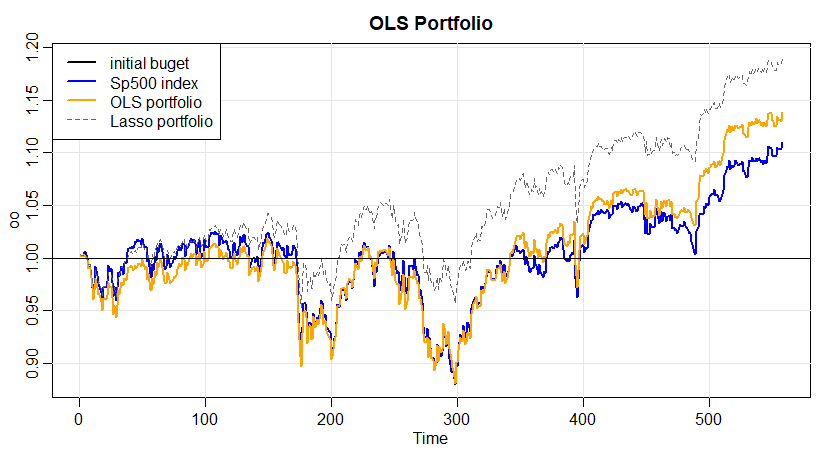
\includegraphics[scale=0.60]{olsportfolio}
\\

Actually also in our case OLS approximate the original index much better that the other two approaches. So at the end of our simulations we would say that at the moment the better strategy to build a portfolio is to use lasso an invest on the selected assets proportionally to the ols estimate of the corresponding $\beta$. 
With this approach at the end we gain less that using the others, but this can't be proved to be a general characteristic. Here it happen that lasso and elastic net suggest to invest more on the assets that in future will grow more that the average, further work on investigating if this behaviour repeats also with other indexes would be interesting.

\subsubsection{Dynamic models}

Simulations in the previous section underline that as the time goes our prediction get worth. This is due to the fact that our investment is static while real $\beta$ are dynamic, indeed as the time pass one important asset in the first window can become irrelevant after some lags. Due to this fact it's clear that to better fit the $Sp500$ index one would need update the model.

To show how variable the ideal portfolio is in time we mooved the 250 observation long window trough the dataset, estimating each time a lasso model. What follows is the plot containing the time series of all the asset parameters that are at least ones bigger than zero.
\\

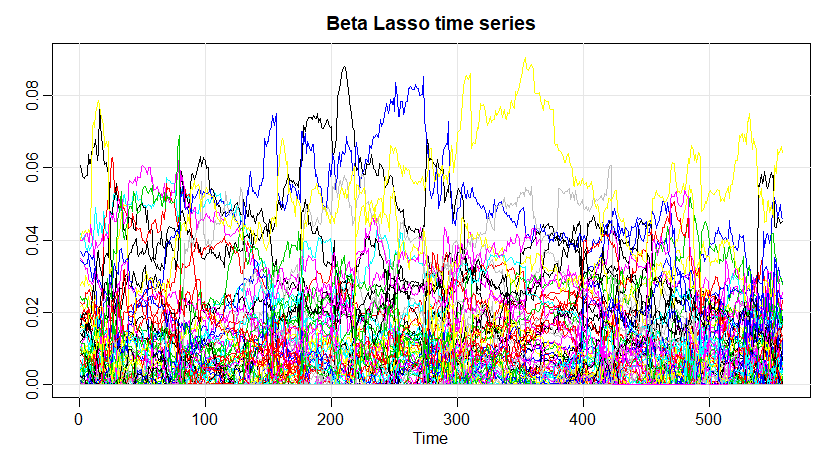
\includegraphics[scale=0.60]{betatime}
\\

This plot seems to be confusing, but actually this is really due to the variability of the beta over the time. One guess we can take from this plot is that even if on average we have 51 assets included in the portfolio, there are only few of them with high beta score, and also there are only few assets which strongly influence the portfolio over the whole analysed time period. Data proves that the intuition was right, indeed we have on average only 11 assets with related beta bigger then 0.023. 

Actually the time variance importance of the assets resulted to be quite relevant. Indeed we built a dynamic regression model using the Kalman filter and we found that also with a dynamic model with only 14 assets, the performances where similar to the lasso approach, which considers 47 assets. This underlign the importance of time in this framework.

Below the plot of the index and our portfolio value over time.
\\

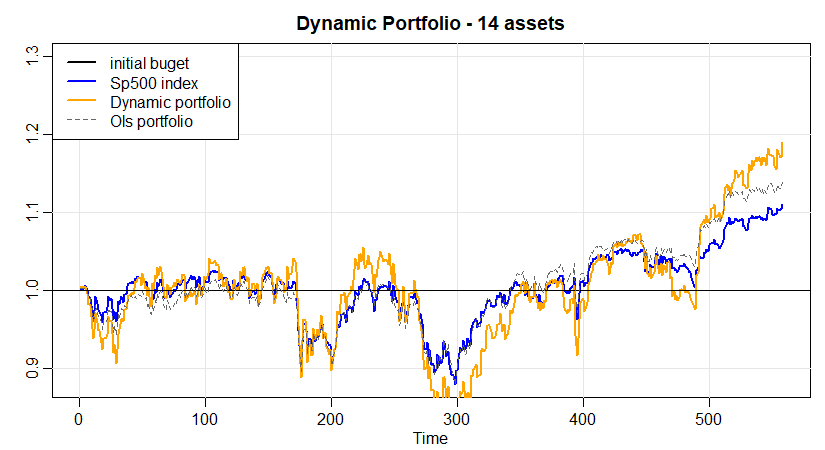
\includegraphics[scale=0.60]{dynamic14}
\\

In general we also built a dynamic model with the same 47 assets considered by the lasso model. This sounds to be perfect, theoretically we should get a perfect fit and should be the ideal solution to portfolio replication problem. The problem with this model is actually the same characteristic that makes it  good at prediction: the frequency of update. Indeed every time one update the model, in real life, should pay a fee due to the new investment, and the daily update of this approach make it unfeasible. Also another reason to doubt this result is its robustness to rapid change in $Sp500$, indeed the Kalman filter we used assumes gaussianity and homoschedasticity, but our objective series is etheroschedastic.  

Below the plot of the Kalman filter results with respect to OLS prediction and $Sp500$.
\\

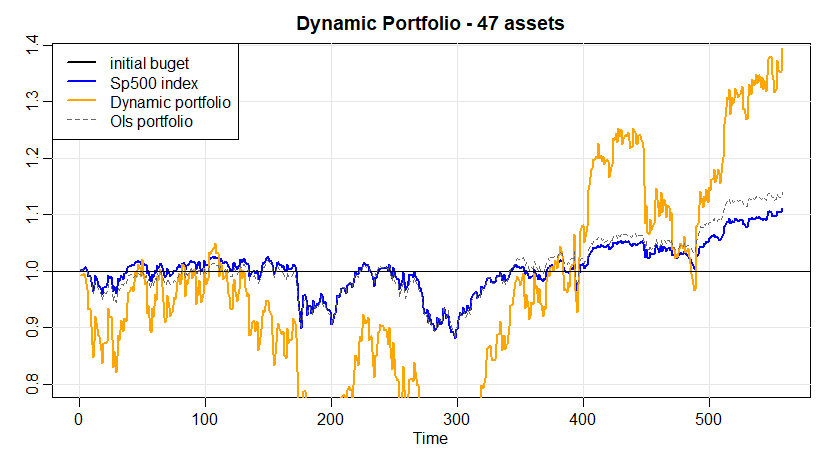
\includegraphics[scale=0.60]{dynamic47}
\\

  
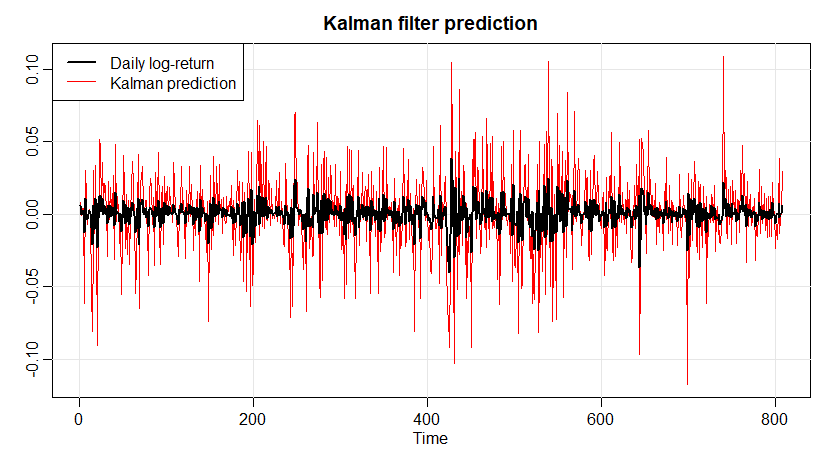
\includegraphics[scale=0.60]{kalmanprediction}
\\       

As we said, here the low robustness of the method end up in really variable prediction. From the second plot it's clear that the homoschedasticity here is not respected and in general we have a really variable series to predict,for this reason this dynamic model is useless.

\subsection{Active approach}
Now we want to try to use our predictions to build up a financial strategy: we invest our money at time $t$  in order to replicate $Sp500$ index only if we think that tomorrow the index will grow, otherwise we capitalize our portfolio and we don't invest money at time $t$. Every day we repeat this procedure trying to guess when the market will go up, investing only if this is the case.  Of course, we must consider a variable fee ($0.2\%$) we need to pay to make an investment.  We can aggregate this tax
to $y$, the daily log revenue, modifying its value $y\rightarrow y+log(1-0.002)$: in this way if the new $y$ is still positive we want to reinvest our money even though this means to pay the additional fee.
\\

We will show below two different approaches: the first one deals with shifted windows to get one-step ahead predictions of the index, the other uses logistic regression to understand if we are in an ascending state or in a descending one.

\subsubsection{One-step ahead prediction with shifted windows}
As seen above we can get the one-step ahead prediction of our $Sp500$ index applying Lasso to shifted windows:
\begin{equation}
 \min_{\beta} \sum_{t=1}^T ( y_{t+1} -\beta_0 -\sum_{j=1}^p x_{tj} \beta_j)^2 ~~subject~to~\sum_{j=1}^p |\beta_j| \leq C.
\end{equation}
We can use this prediction in order to decide if we want to invest, because the index will grow and as consequence also our portfolio replicating it, or save our money. Below we show a simulation where we invest on average into 69 assets and after 
less than 600 days we increase our portfolio by $5\%$. 
\newpage
  \begin{figure}[h!!!!!]
  \centering
  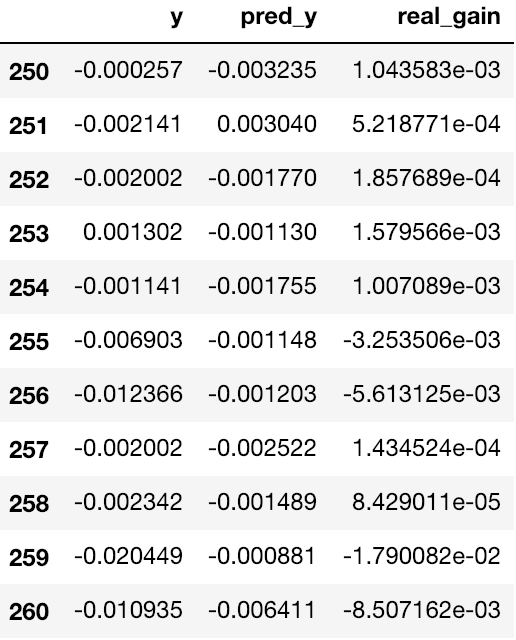
\includegraphics[scale=0.6]{act_port.png}
  \caption{Portfolio's evolution with 69 variables}
  \label{portfolio_alpha}
  \end{figure}
  
    \begin{figure}[h!]
  \centering
  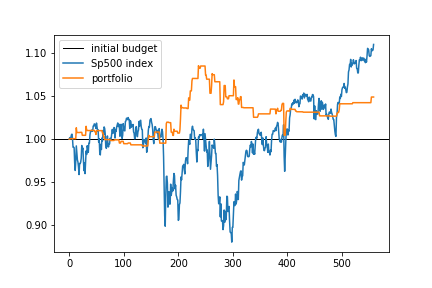
\includegraphics[scale=0.6]{act_portfolio.png}
  \caption{Portfolio's evolution compared with $Sp500$ index}
  \label{portfolio_alpha}
  \end{figure}

As can be seen looking at the graph, with this approach we are able to avoid the fast decrease of the index around $t=150$, on the other hand we can't fully exploit the final growth due to the fees we need to pay every time we decide to rebuild our portfolio.

\subsubsection{Logistic regression}
Since our concern is about predicting every day which is the right choice between reinvest or not the money inside our portfolio we can use a logistic model where if the prediction for day $t$ is $0$ we don't invest our budget at $t$, vice versa if the prediction for day $t$ is $1$ we invest our budget at $t$ according to the $\beta_{Lasso}$ coefficients estimated as before using $X[t-250:t-1]$.

  \begin{figure}[h!]
  \centering
  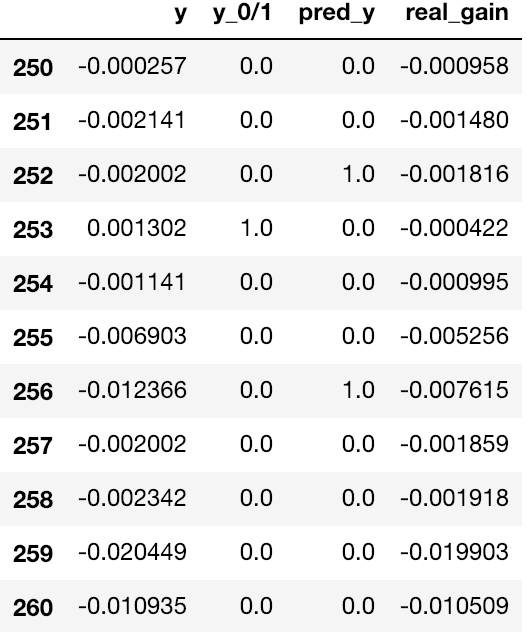
\includegraphics[scale=0.55]{act_port_log.png}
  \caption{Portfolio's evolution with 69 variables}
  \label{portfolio_table_logit}
  \end{figure}
  
      \begin{figure}[h!]
  \centering
  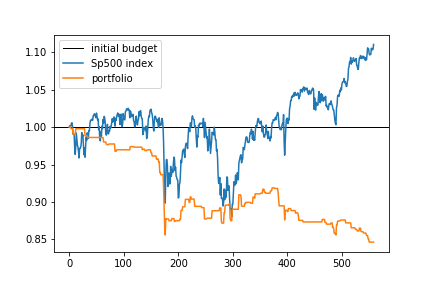
\includegraphics[scale=0.6]{act_portfolio_logit.png}
  \caption{Portfolio's evolution compared with $Sp500$ index}
  \label{portfolio_graph_logit}
  \end{figure}

Looking at the data we can see that our problem here is that we are not able to predict efficiently the value of $Sp500$ index and because of that we end up investing in the wrong moments.


\newpage

\section{Conclusions}

At the end of this work we feel to have a deep understanding of the analysed problem and its field. The work presented here is just a gentle introduction to portfolio management methods, nevertheless we touched a wide range of problems and tried to propose different techniques to deal with them.
\\

The principal aim of this work was to manage and give a possible solution to portfolio replication problem. We  proposed different methods based on active or passive approach.

From our specific analysis if an investor would like to follow an active approach, we would suggest him a non negative lasso model in order to predict the future value of the $Sp500$ index and invest in the selected assets proportionally to a Lasso model built on the most recent available window.

Anyway, in general we would not suggest an active approach. High variability of the index often brings to mispredictions and consequently to losses, considering also that lots of money is spent in taxes while frequently rebuilding our portfolio. Indeed we would go for passive approach. In particular the best available option seems to be a portfolio in which one invest proportionally to OLS beta related to lasso-selected assets.
This approach is much less variable and our results support the evidence underlined quite often in the literature: passive approach seems to bring better results if compared with active approach. 
\\

Again is important to say that this wants to be an example of how one can deal with a portfolio replication problem, and with a different index one would have obtained different results. So it is important to say that what does not allow us to perform well using active approach is that our model for predicting the one-step ahead index return is not accurate. With a better model, active approach, would be able to outperform passive approach. For sure, then, future work could be done in this direction.




\end{document}